\documentclass[../thesis.tex]{subfiles}

\providecommand{\zcut}{z_{\mathrm{cut}}}
\providecommand{\ycut}{y_{\mathrm{cut}}}

\providecommand{\LIPS}{\mathrm{LIPS}}

\providecommand{\cL}{\mathcal{L}}
\providecommand{\cN}{\mathcal{N}}
\providecommand{\cM}{\mathcal{M}}
\providecommand{\cO}{\mathcal{O}}

\providecommand{\su}{\mathfrak{su}}


\setlength{\parskip}{0pt}

\begin{document}
	It will be helpful to first develop a basic level of understanding about the groomed hemisphere mass distribution which we wish to calculate. In order to understand calculations which deal with the strong force, we must first study the theory of quantum chromodynamics (QCD), albeit at a superficial level. This will lead us naturally into a discussion of jet grooming, followed by a discussion of the calculational framework under which we will work, called Soft-Collinear Effective Theory (SCET). Then, after touching briefly on some specific techniques we will use later, we will be ready to start calculating.

\section{Quantum Chromodynamics (QCD)}\label{technical-sec:QCD}
	Recall that, in the Standard Model, quarks and gluons interact with each other via the strong force. The theory of the strong force is called quantum chromodynamics (QCD). In the context of quantum field theory, QCD can be described by the Lagrangian \cite{larkoski_elementary_2019-1}
	\begin{equation}\label{technical-eq:QCD Lagrangian}
		\cL_{\mathrm{QCD}} = -\frac{1}{4} F_{\mu\nu}^a F^{\mu \nu\,a} + \bar \psi i \gamma \cdot D \psi,
	\end{equation}
	where $F_{\mu\nu}^a$ is the Yang-Mills field strength tensor, $\psi$ is a spinor (describing quarks), and $\gamma$ is a particular set of matrices. $D$ is the covariant derivative defined by
	\begin{equation}
		D_\mu = \partial_\mu - i g A_\mu^a T^a,
	\end{equation}
	with $g$ the strong force coupling, $A_\mu^a$ a field describing gluons, and $T^a$ the matrices of the Lie algebra $\su(3)$. The precise details of this theory are not important for our purposes. What is valuable is to contrast the QCD Lagrangian with the Lagrangian of quantum electrodynamics (QED), which describes electromagnetism.\footnote{Electromagnetism is, hopefully, more familiar and intuitive to you than the strong force.} This Lagrangian is \cite{larkoski_elementary_2019-1}
	\begin{equation}\label{technical-eq:QED Lagrangian}
		\cL_{\mathrm{QED}} = -\frac{1}{4} F_{\mu\nu} F^{\mu \nu} + \bar \psi \qty(i \gamma \cdot \partial - m - e\gamma \cdot A)\psi,
	\end{equation}
	where $A_\mu$ is the vector potential of the photon, $\psi$ describes fermions, and $F_{\mu\nu}$ is the electromagnetic field strength tensor. The value $e$ is the electromagnetic coupling (or, from a different perspective, the charge of the electron), and $m$ is the mass of the electron.

	Notice that Eqs.~\ref{technical-eq:QCD Lagrangian} and \ref{technical-eq:QED Lagrangian} are remarkably similar in structure. This hints at a fundamental similarity between the two theories. Both describe particles which carry a charge, as well as a massless force carrier which mediates interactions between particles with charge. In QED, that charge is the familiar electric charge; in QCD, it is called \textbf{color} charge.\footnote{Hence the name quantum \textbf{chromo}dynamics}\footnote{Incidentally, the color charge of QCD has absolutely nothing to do with color as we usually think of it. It is simply a whimsical name.}

	The primary difference between these two theories lies in their field strength tensors. In QED, the field strength tensor is \cite{larkoski_elementary_2019-1}
	\begin{equation}
		F_{\mu \nu} = \partial_\mu A_\nu - \partial_\nu A_\mu.
	\end{equation}
	The result is that, in Lorentz gauge $\partial \cdot A = 0$,
	\begin{equation}
		\partial^2 A^\nu = 0,
	\end{equation}
	which reveals the familiar fact that electromagnetism obeys the principle of superposition \cite{larkoski_elementary_2019-1}. In contrast, the field strength tensor for QCD is \cite{larkoski_elementary_2019-1}
	\begin{equation}\label{technical-eq:QCD field strength}
		F_{\mu \nu}^a = \partial_\mu A_\nu^a - \partial_\nu A_\mu^a + g f^{abc} A_\mu^b A_\nu^c.
	\end{equation}
	Here, $f^{abc}$ are the structure constants of the $\su(3)$ algebra. Notice that the QCD field strength tensor has a third term relative to the QED field strength tensor. This term is quadratic in the gluon field, with the result that QCD is a highly nonlinear theory \cite{larkoski_elementary_2019-1}. 

	Physically, this means that gluons interact with themselves! This is a bizarre property which makes makes QCD simultaneously difficult to work with and very rich in structure. We will see a direct manifestation of this phenomenon in Sec.~\ref{technical-sec:jets}.

\subsection{Approximate scale invariance}
	For our purposes, one of the most important consequences of the structure of the QCD Lagrangian is that the theory is (approximately) scale invariant. What this means is that, if we shift the energy scale of a system governed by QCD, its dynamics are unchanged. 

	To see this, one can observe the action of the QCD Lagrangian under a scale dilation $x^\mu \to \lambda x^\mu$. In the limit of massless quarks, the QCD action is \cite{larkoski_elementary_2019-1}
	\begin{equation}
		S[A_\mu^a, \psi] = \int d^4 x \qty[-\frac{1}{4} F^a_{\mu \nu}F^{\mu\nu\,a} + \bar\psi i \gamma \cdot D \psi].
	\end{equation}
	Under the dilation $x^\mu \to \lambda x^\mu$, the action transforms as \cite{larkoski_elementary_2019-1}
	\begin{equation}
	\begin{aligned}
		S[A^a_\mu, \psi] &\to \int d^{4}x \lambda^4 \qty[-\frac{1}{4} \lambda^{-2} F^{a}_{\mu\nu}\lambda^{-2}F^{\mu\nu\,a} + \lambda^{-3/2}\bar \psi i \gamma \cdot D \lambda^{-1} \psi \lambda^{-3/2}] \\
		&= S[A_\mu^a, \psi].
	\end{aligned}
	\end{equation}
	Scale invariance is another remarkable feature of QCD, which will become important in Sec.~\ref{technical-sec:jets}.

	You will notice, however, that we said the scale invariance is only approximate. That is because the argument outlined above depends on the assumption that the strong coupling $g$ in the field strength tensor, Eq.~\ref{technical-eq:QCD field strength}, is a constant. It turns out that this is not the case. For quantum mechanical reasons, the coupling of the strong force is affected by the temporary production of virtual particles; at different energies, these effects result in different corrections. This is known as the \textbf{running coupling} of the strong force.\footnote{The same effect actually occurs in QED, with the provocative result that the charge of the electron, as we typically conceive of it it, is not actually constant.} For an intuitive description of the mechanics of this effect, see Ref.~\cite{larkoski_elementary_2019-1}.

	We need to take into account the running of the strong coupling when we perform calculations in QCD. Defining the strong coupling to be
	\begin{equation}
		\alpha_s = \frac{g^2}{4\pi},
	\end{equation}
	the running of the coupling is described by the $\beta$-function, defined by \cite{larkoski_elementary_2019-1}
	\begin{equation}
		\beta(\alpha_s) = \mu \frac{\partial \alpha_s}{\partial \mu}
	\end{equation}
	for an energy scale $\mu$. The $\beta$-function can be computed perturbatively in $\alpha_s$; more information about this, including specific values, is given in Sec.~\ref{all-sec:solving RGE}. Where the running of the strong coupling is important, we will write $\alpha_s(\mu)$ to mean the coupling at a particular scale.

	While the running of the strong coupling is an important effect for precision calculations, its effect is small at high energies, so we can still consider QCD to be scale invariant to a reasonable degree of accuracy.

	As remarkable as scale invariance is, it has a significant downside from the perspective of QCD calculations. Many calculations of interest, like the distribution of groomed heavy hemisphere jet masses which we will calculate, impose scales onto the theory (such as the scale of the energy cutoff in jet grooming). In a sense, when one tries to impose a scale onto a scale-invariant theory like QCD, the theory fights back. Logarithms of ratios of scales emerge in the calculation that can grow very large if the scales are far apart, and it is important to account for these effects \cite{larkoski_elementary_2019-1,becher_introduction_2015-1}. Our calculation will use the technique of \textbf{resummation} to account for these large logarithms in a consistent manner.

\section{Groomed heavy hemisphere mass}
	Now that we have a basic understanding of the theory of QCD, it is time to learn what we are trying to study.

\subsection{Jets}\label{technical-sec:jets}
	Two oddities of QCD discussed in Sec.~\ref{technical-sec:QCD} --- the gluon self-interaction and the scale invariance of QCD --- conspire to generate a unique experimental phenomenon called \textbf{jets}. As a high-energy quark or gluon propagates, it radiates gluons, which in turn might produce quark-antiquark pairs, which then radiate gluons, and so on. Because QCD is scale invariant, as we `zoom in' on the emissions,\footnote{By changing either the length or the energy scale} we will see the same structure emerge at all scales. That is, when a color-charged particle is produced at high energy, there will be an arbitrary number of emissions alongside that particle \cite{larkoski_elementary_2019-1}. 

	As we discussed above, however, QCD is not truly scale-invariant, and as more particles are emitted the energy of each individual particle decreases. Eventually, the energy falls to the \si{\giga\electronvolt} scale and below, at which point \textbf{hadronization} occurs --- quarks and gluons settle into bound states like protons, neutrons, and pions. The end result of all this is that we never see an individual quark or gluon in a detector. Instead, we see collimated streams of these hadronic particles, to which the term `jet' refers.

	\begin{figure}
	\begin{center}
		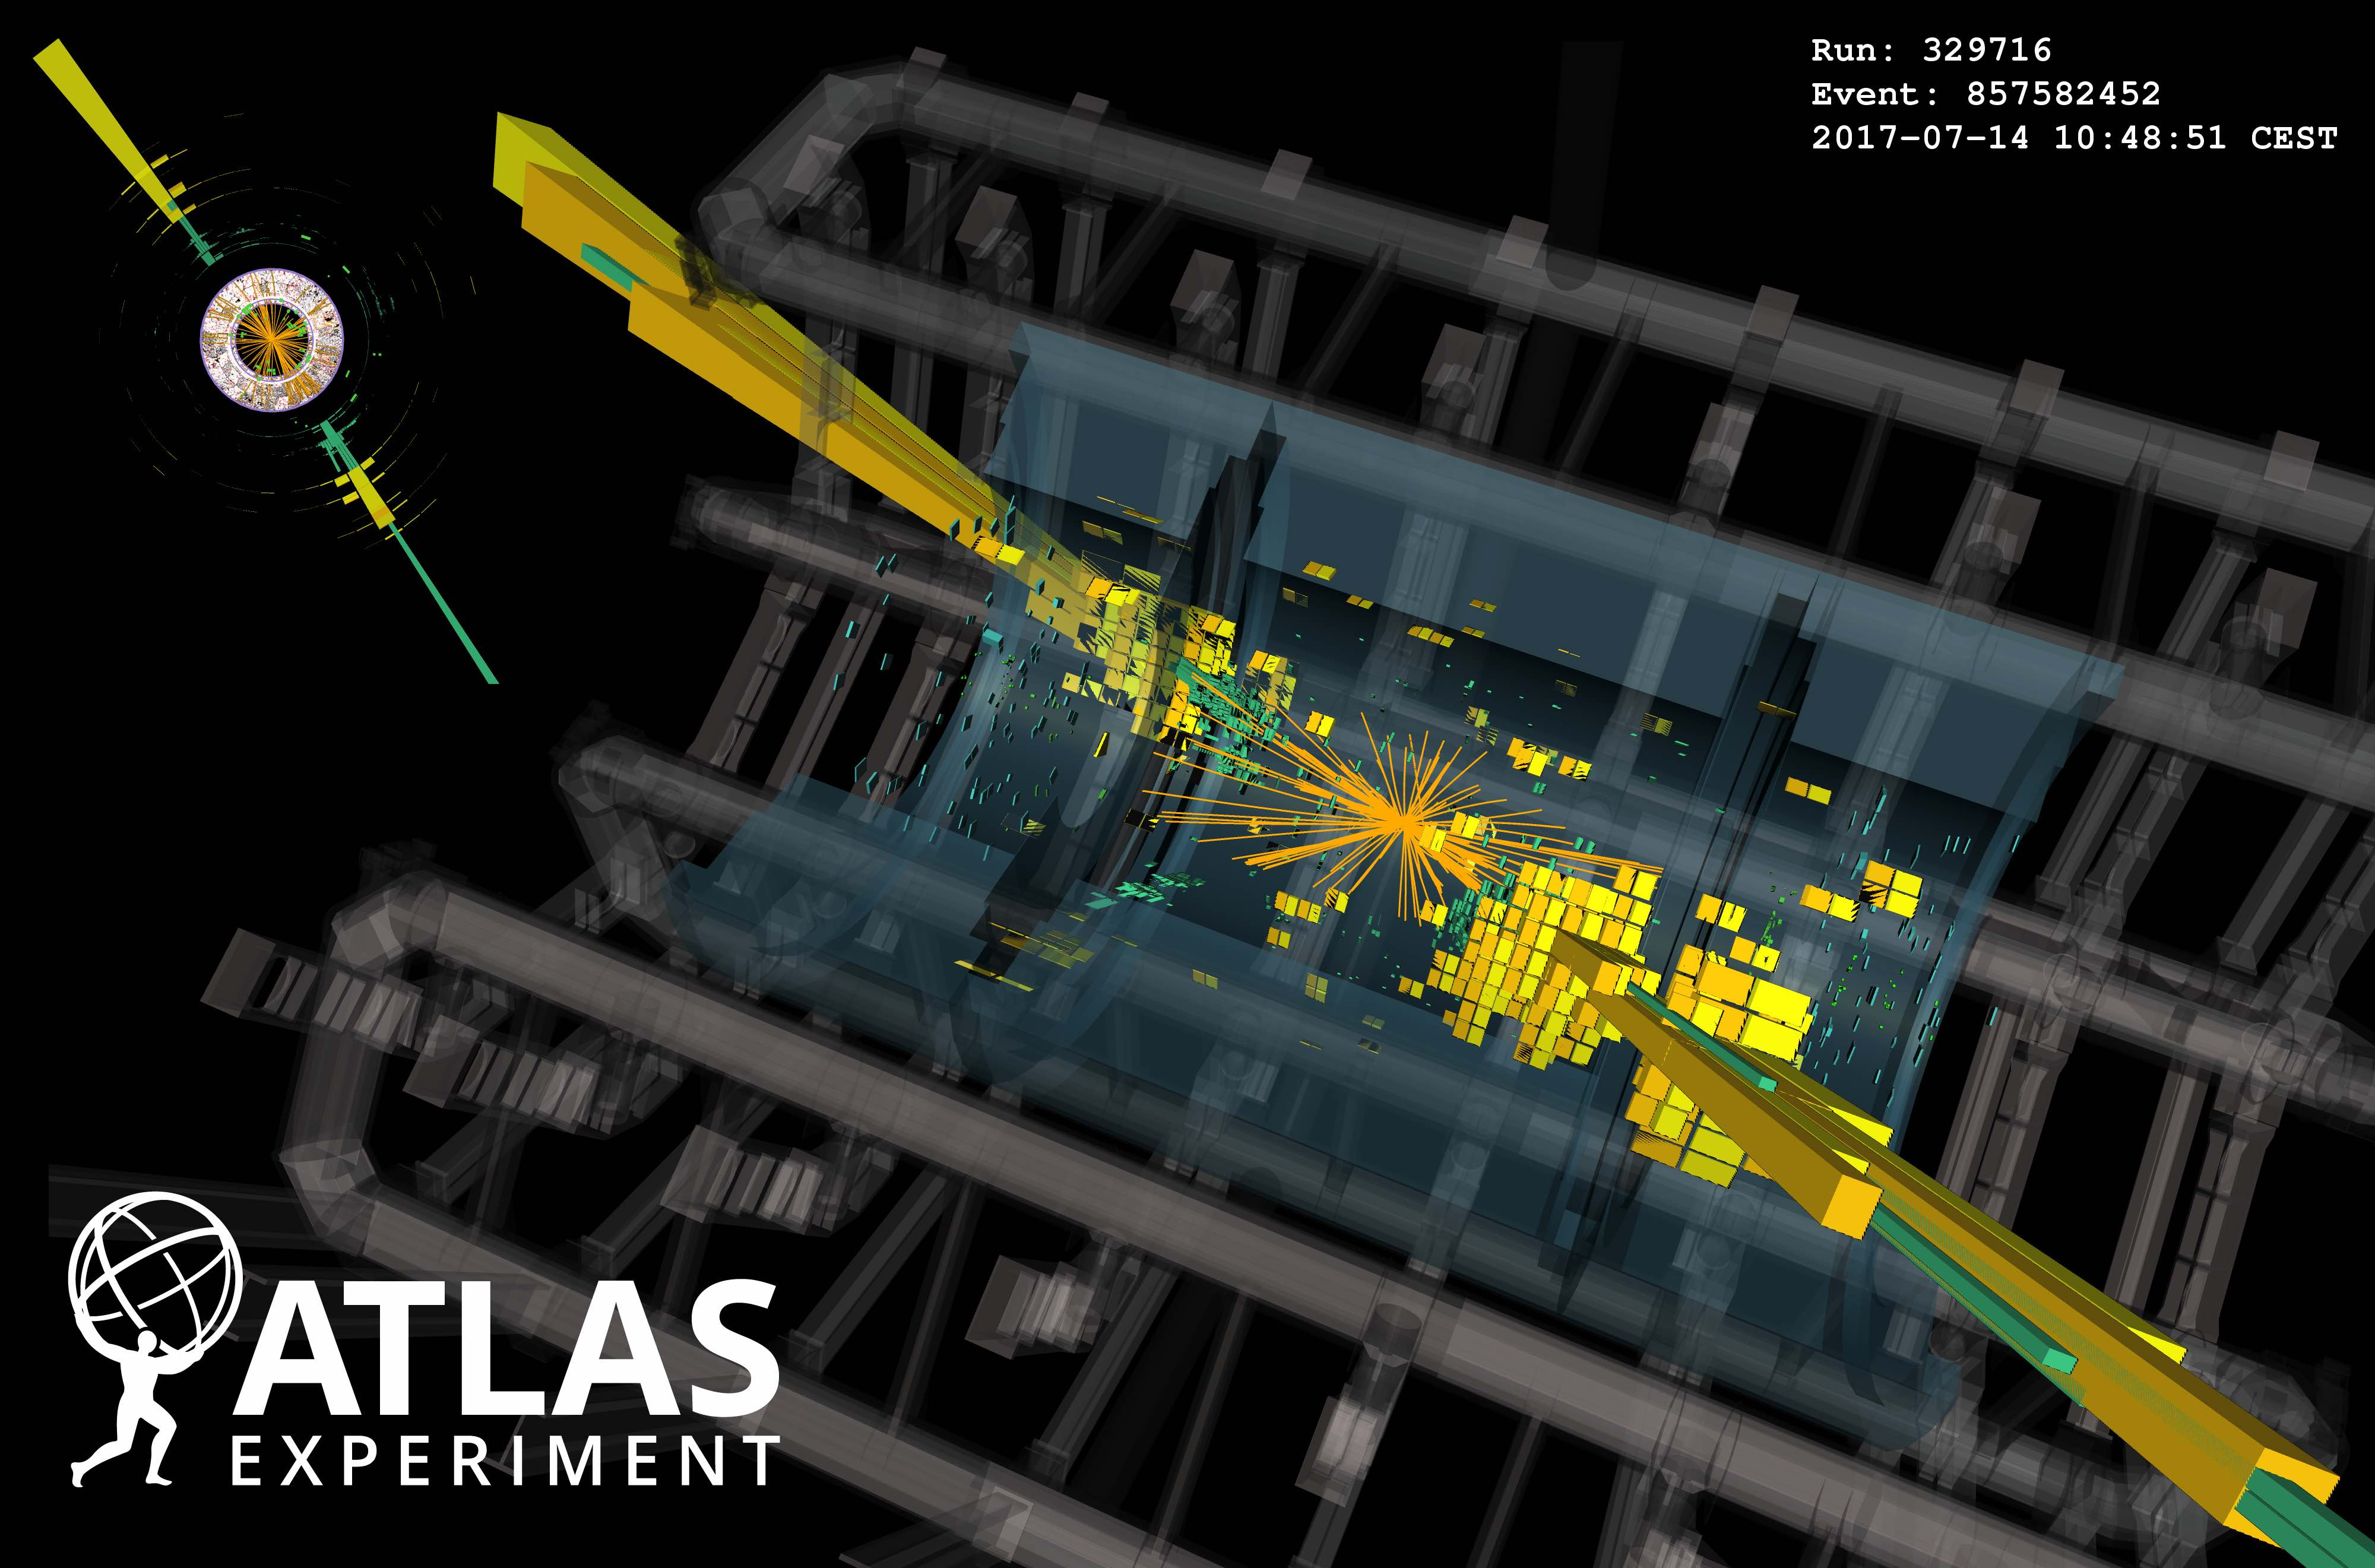
\includegraphics[width=\textwidth]{figures/DijetHighMass9.3TeV-VP1-nocone_small.jpg}
		\caption{\label{technical-fig:dijet}An event captured by the ATLAS detector in 2017 in which two jets are produced. From \cite{atlas_collaboration_event_nodate}}
	\end{center}
	\end{figure}

	Figure \ref{technical-fig:dijet} shows an example of the production of two jets in a proton-proton collision in the ATLAS experiment at the Large Hadron Collider. The solid bars represent particle energies measured in the hadronic calorimeter. Notice that the energy is deposited in strongly collimated streams, as predicted.

\subsection{Cross sections}
	We would like to compute properties of jets in electron-positron collisions. But what are the actual objects we can work with?

	In high-energy physics, the standard experimental strategy is to perform many particle collisions, observe the results of each collision, and then make observations about these results \textit{en masse}. Because of the probabilistic nature of quantum mechanics, there is little to be learned from individual events. Instead, questions in the field require statistical answers drawn from massive datasets.

	One basic question one could reasonably ask in this context is ``What is the probability of event $X$ occurring?'' We describe this probability as a \textbf{cross section} $\sigma(X)$.\footnote{The origin of the term comes from early experiments which measured the probability of two particles colliding with or scattering off of each other. The term `cross section' was an attempt to draw an analogy to the classical problem of two macroscopic objects colliding. The probability that they will hit each other is proportional to their cross-sectional area.} Cross sections are measured in units of area called \textbf{barns}, with $\SI{1}{\barn} = \SI{10E-24}{\squared\centi\meter}$.\footnote{The origin of the unit `barn' comes from the Manhattan project, where the problem \textit{du jour} was to calculate the probability that neutrons would, say, cause fission events in materials like uranium. It turns out that the probability of neutron absorption by U-235 is on the order of \SI{1}{\barn}, and this probability was deemed to be `as big as a barn'. There is another side to the story involving unfortunate names and bathroom humor, which can be read in Ref.~\cite{holloway_how_1972}.}

	If it is not interesting enough to measure the probability of a specific process occurring, one might instead ask about the distribution of a cross section over a particular observable. If we want to measure the distribution of $x$ in a collision event, then we could measure the \textbf{differential cross section} $d\sigma/dx$. If cross sections are essentially probabilities, then differential cross sections are probability distributions --- they tell us the probability of that the variable $x$ will take on a set of values. Integrating over $x$ would return the total cross section $\sigma$.

	Cross sections can be either inclusive or exclusive. An \textbf{inclusive} cross section is one which allows for a particular event \textit{alongside anything else}. For example, suppose we are interested in the production of a quark-antiquark pair in electron-positron collisions, but do not care if additional particles are produced:
	\begin{equation}
		e^+ e^- \to q \bar q + X
	\end{equation}
	for some arbitrary particles $X$. Then the cross section $\sigma(e^+ e^- \to q \bar q + X)$ is inclusive \cite{larkoski_elementary_2019-1}. The production of additional particles comes with reduced probability, so the inclusive cross section is a reasonable approximation for the event $e^+ e^- \to q \bar q$. 

	On the other hand, suppose that we wanted to perform precision studies of quark production in electron-positron annihilation and therefore demand that other particles the final state have certain features
	\begin{equation}
		e^+ e^- \to q \bar q + \qty(\text{particles with certain qualities}).
	\end{equation}
	These demands result in a restriction of the allowed phase space of final states, so we call this an \textbf{exclusive} cross section. It becomes important to account for all energy scales imposed by these restrictions --- it is these energy scales which can give rise to large logarithms which must be resummed \cite{larkoski_elementary_2019-1}. 

	Cross sections can be computed using \textbf{Fermi's Golden Rule} \cite{larkoski_elementary_2019-1,schwartz_quantum_2014},
	\begin{equation}\label{technial-eq:Fermi golden rule total}
		\sigma = \cN \int d\Pi_\LIPS \abs{\cM}^2,
	\end{equation}
	where $\cN$ is a normalizing constant. $d\Pi_\LIPS$ is called the Lorentz-invariant phase space measure. It ranges over all the possible four momenta of the $n$ final-state particles, each with momentum $p_i^\mu$. It is defined to be
	\begin{equation}
		d\Pi_\LIPS = (2\pi)^4 \delta^4\qty(P - \sum_{i = 1}^n p_i) \prod_{i = 1}^n \frac{d^4 p_i}{(2\pi)^3} \delta\qty(p_i^2 - m_i^2),
	\end{equation}
	where $P$ is the total four-momentum of the initial-state particles. The first Dirac delta function enforces conservation of momentum, while the second enforces that every final-state particle is \textbf{on-shell}, meaning essentially that it is real. An on-shell particle with momentum $p$ and mass $m$ satisfies $p^2 = m^2$.\footnote{It is possible, quantum mechanically, for particles to exist for a brief period of time \textit{off-shell}. We call these virtual particles, and they are important for high-order corrections in many calculations. In fact, it is these off-shell virtual particles which generate the running of the strong coupling $\alpha_s$.}

	The last term in Eq.~\ref{technial-eq:Fermi golden rule total} is called the $S$-matrix element, or, more commonly, just the \textbf{matrix element}. The $S$-matrix is the scattering matrix which encodes all possible transitions from an initial state to a final state \cite{larkoski_elementary_2019-1}. Thus, for initial-state particles $p_1^i, p_2^i, \dots, p_m^i$ and final-state particles $p_1^f, p_2^f, \dots, p_n^f$, the matrix element is
	\begin{equation}
		\braket{p_1^i p_2^i \cdots p_m^i}{p_1^f p_2^f \cdots p_n^f}.
	\end{equation}

	While Eq.~\ref{technial-eq:Fermi golden rule total} allows for the calculation of a total cross section, it must be slightly modified to compute a differential cross section. To measure an observable $x$, we must introduce a measurement term of the form
	\begin{equation}
		\delta_x = \delta\qty(x - f(p_1, p_2, \dots, p_n))
	\end{equation}
	where $f(p_1, p_2, \dots, p_n)$ is a function of the final-state momenta. Integrating over this delta function inserts the observable in place of the function $f$ of the momenta. Thus, the version of Fermi's Golden Rule which we will use is
	\begin{equation}\label{technical-eq:Fermi golden rule differential}
	\boxed{
		\frac{d\sigma}{dx} = \cN \int d\Pi_\LIPS \abs{\cM}^2 \delta_x.
	}
	\end{equation}

\subsection{Heavy hemisphere mass}
	One of the most basic properties of anything is its mass, so it is reasonable that we might want to know the distribution of possible jet masses. This can both provide information about the physics of jets and assist in precision measurements of quantities like the strong coupling $\alpha_s$.

	Although the state-of-the-art collider, the LHC, collides protons on protons, this experimental arrangement is problematic for precision measurements.\footnote{Though it is excellent for the discovery of new particles, which was the founding mission of the LHC.} Protons are composite particles --- each consists of two up quarks and one down quark --- and when they collide it is impossible to know even which fundamental particles interacted with which other particles, let alone to know their momenta or energies. In short, proton-proton collisions are a (useful) mess. By contrast, electrons and positrons are fundamental particles, and parameters of their collisions can be very well-controlled in colliders. For these and other reasons, electron-positron collisions are viewed as the ultimate precision tool.\footnote{There are other problems, though, namely that synchrotron radiation makes it all but impossible to develop an $e^+ e^-$ collider which could reach energies above a few hundred \si{\giga\electronvolt}. Other leptons have nice collisional properties, though, while their higher mass limits the problems with energy loss during acceleration. For this reason, there is a growing discussion about building a muon-antimuon collider in the coming decades --- if the funding could be found! There are also plenty of technical challenges with this idea that need to be solved first.}

	It also happens (for similar reasons) that electron-positron collisions are much easier to account for theoretically than proton-proton collisions. We are therefore going to consider $e^+ e^- \to \text{jets}$ events.

	We wish to measure the heavy hemisphere mass $\rho$, which will be defined shortly. In the limit $\rho \ll 1$, the leading contribution to the distribution comes from the emission of a back-to-back quark-antiquark pair (such an event is visible in Fig.~\ref{technical-fig:dijet}). The mass of each hemisphere can be measured separately as the sum of all particles in the hemisphere. If hemisphere $i$ has mass $m_i$ and energy $E_i$, the hemisphere mass ratio of interest is defined to be
	\begin{equation}
		\rho_i = \qty(\frac{m_i}{E_i})^2.
	\end{equation}
	The heavy hemisphere mass ratio is simply the larger of the two:
	\begin{equation}\label{technical-eq:rho definition}
	\boxed{
		\rho = \max[\rho_1, \rho_2] = \qty(\frac{m_h}{E_h})^2,
	}
	\end{equation}
	with $m_h$ the mass of the heavier hemisphere and $E_h$ its energy. Our target distribution will be the differential cross section $d\sigma/d\rho$.

\subsection{Jet Grooming}
	The story is not quite done, as we still need to take jet grooming into account. Jet grooming is a primarily experimental technique used to obtain clean data. Particle collisions and measurements do not happen on their own --- since the probability of a collision between particles in a collider is low, the particles are collided in large bunches to ensure at least one collision event per beam crossing. As technology has improved, collision probabilities have been brought higher, which means that an increasing number of collisions happen per crossing. 

	\begin{figure}
	\begin{center}
		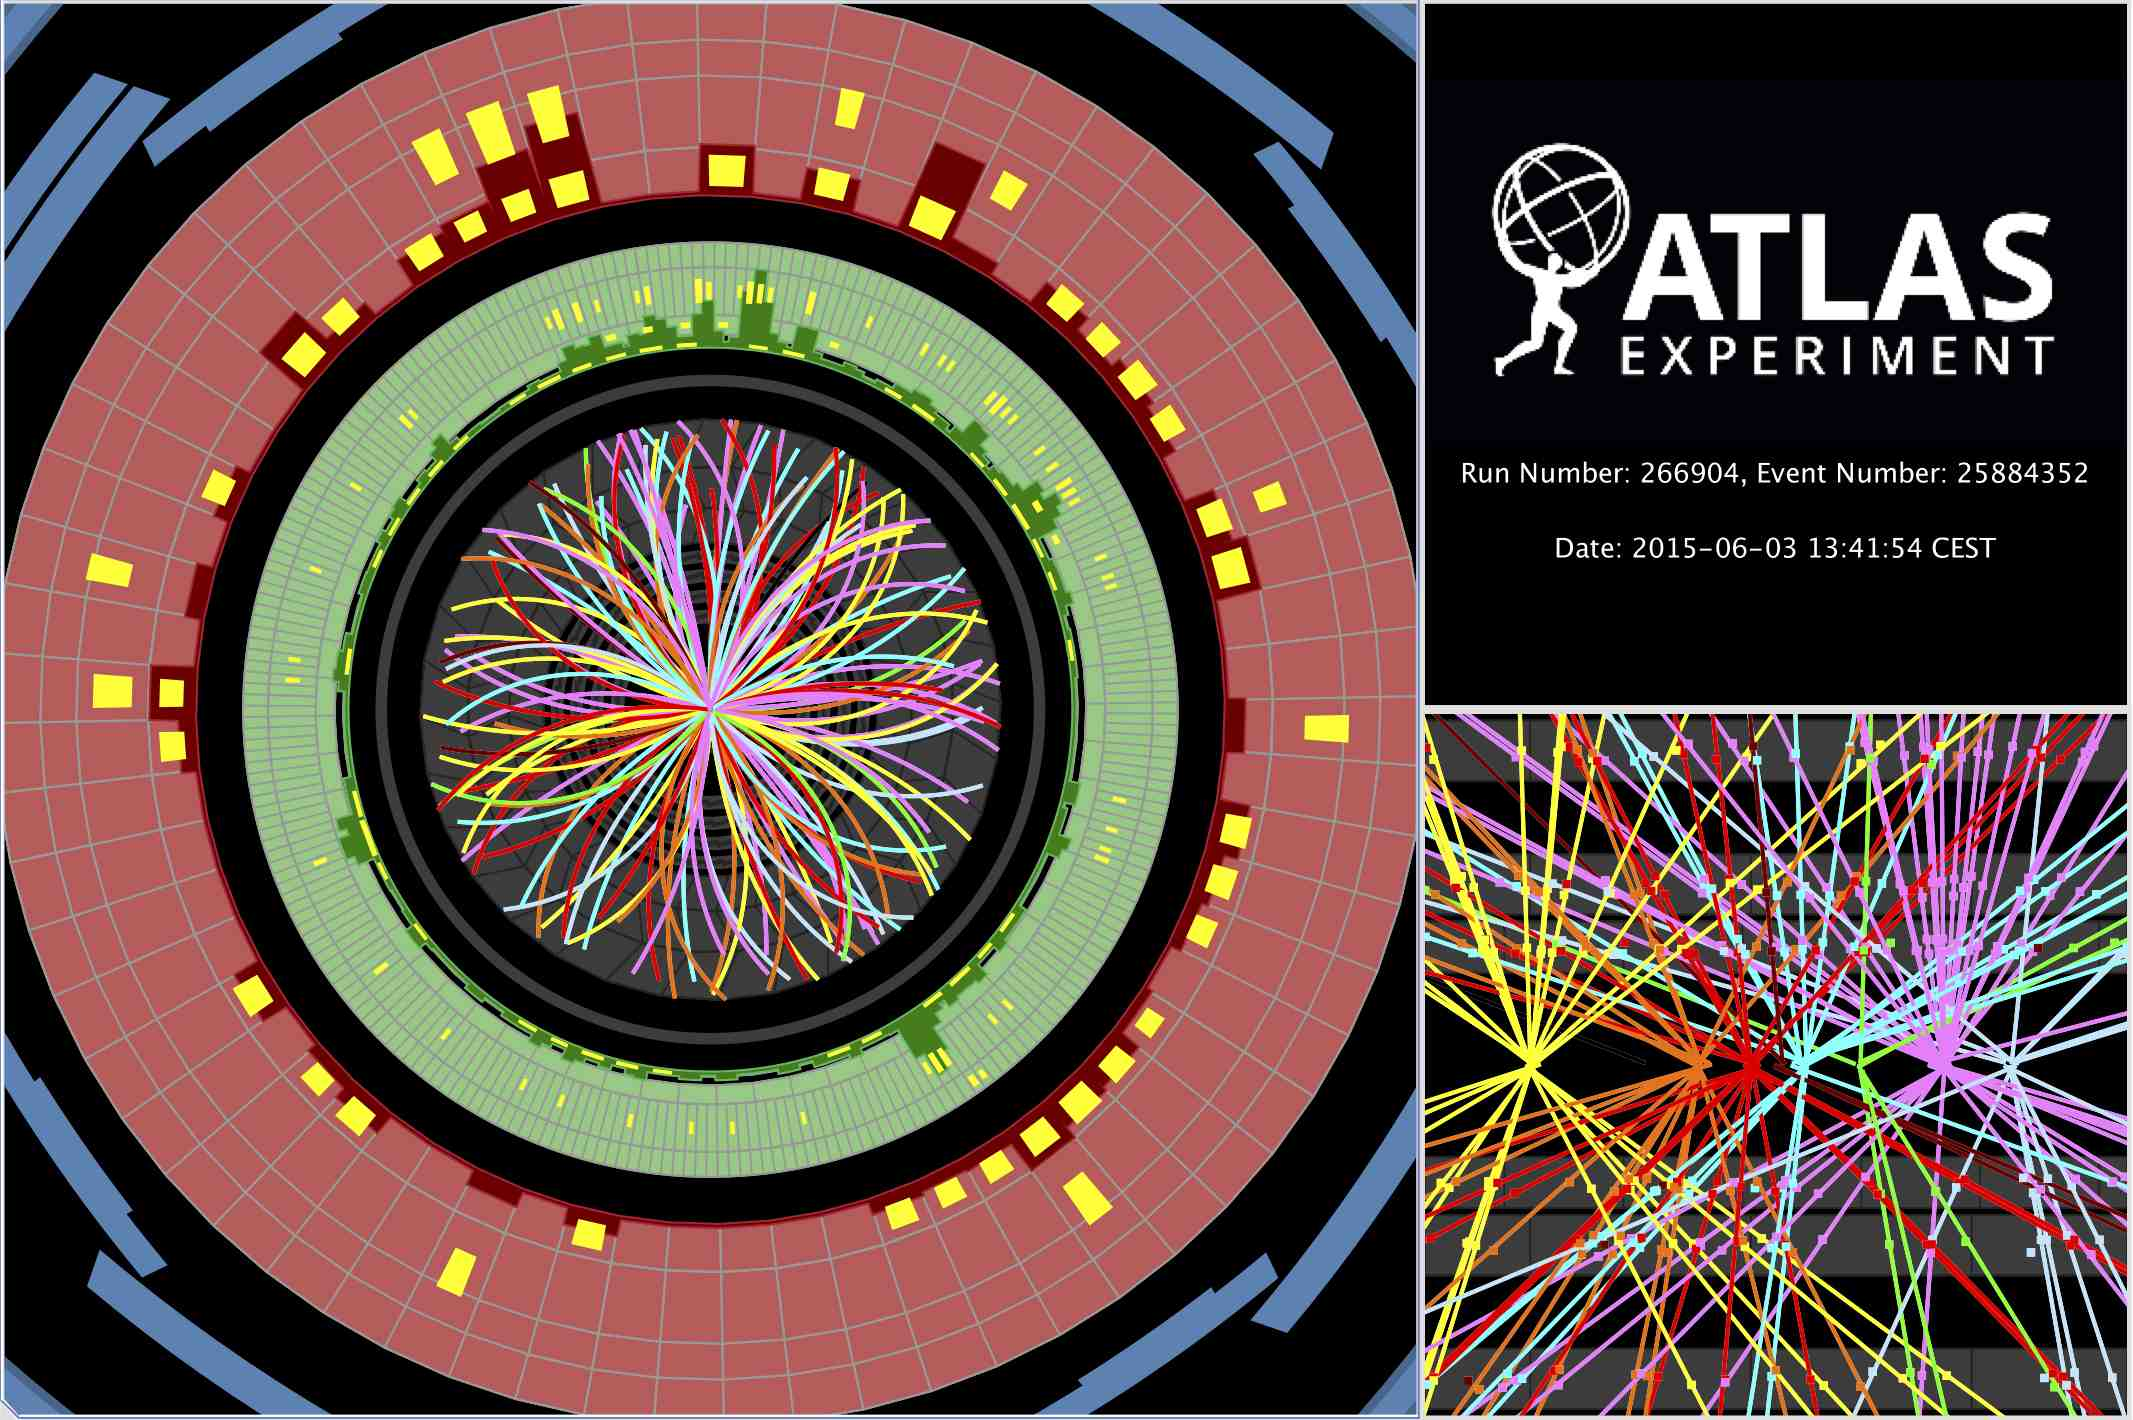
\includegraphics[width=\textwidth]{figures/atlas_pile_up.jpeg}
		\caption{\label{technical-fig:pileup}An event captured by the ATLAS detector in 2015 which exhibits moderate pileup. From \cite{atlas_collaboration_event_nodate-1}}
	\end{center}
	\end{figure}

	When multiple collisions happen simultaneously in the detector, the situation is called \textbf{pileup}. An example of an event with moderate pileup\footnote{In fact, the pileup of this event is fairly low by today's standards. Within the next decade, after the LHC undergoes its High Luminosity upgrade, as many as dozens of collisions could happen per bunch crossing.} is displayed in Fig.~\ref{technical-fig:pileup}. Notice how particles from each interaction stray into other interactions, possibly contaminating data on those interactions. This is not a problem for something like the tracking system, which can reproduce a particle's track to identify which interaction generated it; but for the calorimetry system, which is the primary way to measure jet masses, it is can be very difficult to disentangle these interactions.

	Particle physicists have developed a number of \textbf{jet grooming} techniques to study jet properties while minimizing these effects. The basic idea of a jet groomer is to cut away particles with undesirable properties.

	We will focus on one, which is a slightly modified version of the Modified Mass Drop Tagger (mMDT) \cite{dasgupta_towards_2013}. The algorithm is as follows \cite{kardos_two-_2020}:
	\begin{enumerate}
		\item Divide the event into two hemispheres 

		\item For each hemisphere, run the Cambridge/Aachen jet algorithm \cite{dokshitzer_better_1997,wobisch_hadronization_1998}:
		\begin{enumerate}
			\item Create a table $T$ of the energies $E_i$ of particles and an ordering variable $R_{ij}^2 = \Delta \eta_{ij}^2 + \Delta \phi_{ij}^2$, where $i$ and $j$ range over all particles, $\phi$ is the azimuthal angle, and $\eta$ is pseudorapidity.\footnote{Pseudorapidity is defined as 
			\begin{equation} \eta = -\log(\tan\frac{\theta}{2}), \end{equation} where $\theta$ is the polar angle from the beam axis. As the angle of the particle approaches the beam axis, $\eta \to \infty$.} Set some cutoff $R_0$.

			\item If $T$ contains only one item, store this item as a jet and return the jets

			\item Select particles $(i, j)$ which minimize $R^2_{ij}$

			\item Do the following:
			\begin{itemize}
				\item If $R^2_{ij} < R_0$, delete $i$ and $j$ from $T$. Create a new particle $(ij)$ with momentum $p_{ij} = p_i + p_j$, recompute relevant values of the ordering variable, and add $(ij)$ to $T$

				\item If $R^2_{ij} \ge R_0$, store $i$ and $j$ as jets and delete them from $T$
			\end{itemize}

			\item Repeat, starting at step (b)
		\end{enumerate}
		In summary, the Cambridge/Aachen algorithm clusters sequentially particles by angular proximity.

		\item Pick some $0 \le \zcut < 1/2$. Starting in one hemisphere at the widest angle, iterate through the pairs of particles (or sets of particles) returned in step (2). For each pair of particles $i, j$, test whether
		\begin{equation}
			\frac{\min\qty[E_i, E_j]}{E_i + E_j} > \zcut.
		\end{equation}
		If it is true, stop and return all particles remaining in the hemisphere. If not, remove the lower energy set of particles. Repeat this step until the hemisphere passes the cut.

		\item Repeat step (3) for the other hemisphere.
	\end{enumerate}
	The intuition behind the mMDT groomer is that it removes particles whose energy fraction falls below $\zcut$, unless the particles are at a smaller angle than one which passed the cut. Most stray background radiation will appear with low energy at a wide angle relative to the core of the jet --- an mMDT groomer removes this radiation.

	Of course, we also run the risk that some of the radiation from the jet itself will be cut by the groomer. That is why we need to calculate the jet mass distribution in the presence of mMDT grooming, since the groomer will modify the shape of the ungroomed distribution. High-precision calculations have already been performed in the limit $\rho \ll \zcut \ll 1$ \cite{frye_factorization_2016,kardos_groomed_2020,kardos_two-_2020}, as well as at fixed order (which is accurate for large $\rho$) \cite{kardos_soft-drop_2018}. As of yet, the distribution is not well-understood in the limit $\rho \sim \zcut \ll 1$, though this is an important region physically, as the relative size of the two scales is no longer dramatically different \cite{larkoski_improving_2020}. This, then is the goal:\\

	\noindent\fbox{%
    	\parbox{\textwidth}{%
        	We wish to calculate the differential cross section $d\sigma/d\rho$, with $\rho$ defined by Eq.~\ref{technical-eq:rho definition}, in $e^+ e^- \to \text{jets}$ events in the presence of mMDT grooming. We will work in the limit $\rho \sim \zcut \ll 1$.
    	}%
	}
	
	\,\\

	While it might be reasonable to worry that the grooming algorithm will make the calculation more difficult (it introduces another external scale $\zcut$, after all), it turns out that there are theoretical benefits to jet grooming, in addition to the experimental ones. A common problem in the calculation of jet observables is the presence of \textbf{non-global logarithms}, which are large logarithms of scales from radiation external to the jet.\footnote{This is the theoretical justification for hating background radiation.} This could be, for example, due to background radiation which radiates particles into the jet as it passes. The presence of non-global logarithms has made it difficult to compute the ungroomed jet mass distribution to high accuracy \cite{dasgupta_towards_2013}. However, it turns out that mMDT grooming eliminates the radiation which could give rise to non-global logarithms, which enables us to achieve higher accuracy than might otherwise be feasible \cite{dasgupta_towards_2013, frye_factorization_2016}.

	This is not the only benefit. It also turns out that the groomed jet mass is more sensitive to the strong coupling $\alpha_s$ than the ungroomed version \cite{larkoski_improving_2020}. If our goal is to measuring $\alpha_s$ using jet masses --- and this would be a valiant goal, as it would be a novel way to measure the coupling and therefore a strong verification of the Standard Model --- then this provides another reason to be interested in the groomed distribution.

	Thus, though we may gain some degree of complication in our calculation from the grooming algorithm, it is well worth the cost. Now let us figure out how to compute it.


\section{Calculational techniques}
\subsection{Soft-Collinear Effective Theory (SCET)}
	The machinery of quantum field theory is, in some sense, too powerful. While the theory is extremely effective at predicting observations in nature, it is also unwieldy. Getting from the QCD Lagrangian of Eq.~\ref{technical-eq:QCD Lagrangian} to a precision calculation of the groomed heavy hemisphere mass would be simultaneously very difficult and not very enlightening.

	Luckily for us, QCD simplifies in the low-energy, or \textbf{soft}, limit in which we will be working (since we are taking $\rho \ll 1$). In this limit, we can replace QCD with a low-energy effective theory called Soft-Collinear Effective Theory (SCET) \cite{bauer_summing_2000,bauer_effective_2001,bauer_invariant_2001,bauer_soft-collinear_2002,beneke_soft-collinear_2002,beneke_multipole-expanded_2003,hill_spectator_2003}. The precise details of SCET are unimportant for our purposes --- for more information, see Refs.~\cite{schwartz_quantum_2014} or \cite{becher_introduction_2015-1}.

	What we will use is the framework which SCET provides for factorizing cross sections. In general, the differential cross section for an $e^+ e^- \to \text{3 jets}$ event takes on a factorized form like \cite{ellis_jet_2010,frye_factorization_2016}
	\begin{equation}
		\frac{d^2\sigma}{d\rho_1 d\rho_2} = H(Q^2) \otimes S(\rho_1, \rho_2, \zcut) \otimes J_q(\rho_1) \otimes J_g(\rho_1, \zcut) \otimes J_{\bar q}(\rho_2),
	\end{equation} 
	where here $\rho_1$ and $\rho_2$ are the normalized masses of the two hemispheres. $H(Q^2)$ is a hard function describing $e^+ e^- \to \text{jets}$; $S(\rho_1, \rho_2, \zcut)$ is a function describing soft radiation; and the $J_i$ are jet functions describing the production of collinear radiation in a jet about particle $i$ (in this case, $i$ could be a quark $q$, antiquark $\bar q$, or gluon $g$).

	This factorization will be key for developing an all-orders calculation of the groomed heavy hemisphere mass, as it enables us to resum large logarithms. Much more on the factorization theorem will be discussed in Chapter \ref{chap:factorization}.

\subsection{Dimensional regularization}
	Beyond the framework of SCET, we will work using a technique called \textbf{dimensional regularization}.\footnote{Developed by 't Hooft and Veltman in the 1970s \cite{t_hooft_regularization_1972}} At its heart, dimensional regularization is a scheme for analytically isolating the divergences in divergent integrals. 

	This is done by decreasing the dimension of the calculation by some small amount $\epsilon > 0$ --- we will work in $d = 4 - 2\epsilon$ dimensions instead of the usual $4$. The effect is to siphon divergences in the original integral into poles at $\epsilon = 0$. The result is still divergent if we send $\epsilon \to 0$, but now it is contained in a single term which can be manipulated and possibly removed. Effectively, dimensional regularization provides one answer the question: ``How can we, in a self-consistent way, remove divergences which cancel?''

	As an example, take the integral
	\begin{equation}
		\int_1^\infty \frac{dx}{x}.
	\end{equation}
	This integral is, of course, divergent in one dimension. But now suppose we choose to work in $d = 1 - \epsilon$ dimensions. The integral becomes (ignoring the normalization)
	\begin{equation}
		\int_1^\infty \frac{dx}{x} \to \mu^\epsilon \int_1^\infty \frac{dx}{x^{1 + \epsilon}}
	\end{equation}
	for some arbitrary scale $\mu$. The scale $\mu$ is necessary because the original integral is dimensionless, so the dimension carried by the new $x^{-\epsilon}$ term must be eliminated. Now performing the integral yields
	\begin{equation}
		\mu^\epsilon \int_1^\infty \frac{dx}{x^{1 + \epsilon}} = \frac{\mu^\epsilon}{\epsilon} = \frac{1}{\epsilon} + \log \mu + \epsilon \log^2 \mu + \cO(\epsilon^2).
	\end{equation}
	Notice that the divergence has emerged as single term: $1/\epsilon$. Now if there were another term in the calculation which, when expanded in $\epsilon$, carried a $-1/\epsilon$, the divergences would manifestly cancel. We could then safely take $\epsilon \to 0$ with a finite result at the end.

	Of course, the examples which we will see in practice are a little more complicated, but the basic strategy is the same. Our first encounter with dimensional regularization in the wild will take place in Chapter \ref{chap:leading order}.

\subsection{Resummation}
	The last piece of technical machinery we will use is the technique of \textbf{resummation}. As we have previously mentioned, the presence of multiple energy scales in certain calculations in QCD results in the emergence of logarithms of ratios of those energy scales \cite{larkoski_elementary_2019-1,becher_introduction_2015-1}. If these scales differ greatly, their ratio will be large, and so will the corresponding logarithms. It is possible, and indeed necessary, to tame these terms by accounting for them at \textbf{all orders}. This is the process of resummation. The actual mechanics will make more sense in context, so we will delay further discussion until Sec.~\ref{all-sec:resummation}.

	We are now ready to put our knowledge to work and start calculating. We will begin, in Chapter \ref{chap:leading order}, with the relatively simple task of deriving a fixed-order distribution for the groomed heavy hemisphere mass. This will give us some physical intuition about the distribution, as well as some practice applying our new calculational techniques. From there, we will proceed to derive an all-orders result in Chapters \ref{chap:factorization} and \ref{chap:all orders}.

\end{document}
